\documentclass[12pt, oneside]{article}
\usepackage[letterpaper, margin=1in, headsep=0.5in]{geometry}
\usepackage[english]{babel}
\usepackage[utf8]{inputenc}
\usepackage{amsmath}
\usepackage{amsfonts}
\usepackage{amssymb}
\usepackage{tikz}
\usetikzlibrary{quotes, angles}
\usepackage{graphicx}
%\usepackage{pgfplots}
%\pgfplotsset{width=10cm,compat=1.9}
%\usepgfplotslibrary{statistics}
%\usepackage{pgfplotstable}
%\usepackage{tkz-fct}
%\usepackage{venndiagram}
\usepackage{multicol}

\usepackage{fancyhdr}
\pagestyle{fancy}
\fancyhf{}
\rhead{\thepage \\Name: \hspace{1.5in}.\\}
\lhead{BECA / Dr. Huson / 10th Grade Geometry\\* 29 November 2018}

\renewcommand{\headrulewidth}{0pt}

\begin{document}
\subsubsection*{Do Now: Triangle angle relationships}
 \begin{enumerate}

\item Solve each equation for $x$, \emph{rounded to the nearest thousandth}.  \vspace{.25cm}
  \begin{multicols}{2}
    \begin{enumerate}
      \item $\displaystyle \tan 32^\circ = \frac{x}{14.2}$
      \item $\displaystyle \cos 32^\circ = \frac{14.2}{x}$
    \end{enumerate}
  \end{multicols} \vspace{4cm}

  \item Given right $\triangle ABC$ with $m\angle C=90^\circ$, $m\angle A = 32^\circ$, and $AC=14.2$.
    \begin{center}
      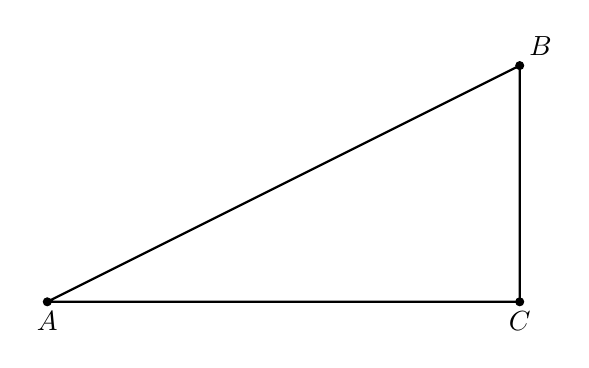
\begin{tikzpicture}%[scale=0.7]
        \draw [thick](0,0)--(6,0)--(6,3)--(0,0);
        \draw [fill] (0,0) circle [radius=0.05] node[below]{$A$};
        \draw [fill] (6,0) circle [radius=0.05] node[below]{$C$};
        \draw [fill] (6,3) circle [radius=0.05] node[above right]{$B$};
      \end{tikzpicture} %\vspace{2cm}
    \end{center}
    \begin{enumerate}
      \item Find $AB$. \vspace{3cm}
      \item Find $BC$. \vspace{3cm}
    \end{enumerate}

\newpage

  \item Given right $\triangle EFG$ with $m\angle G=90^\circ$, $EG=3.3$, $FG=5$, and $EF=6$. Express each trig ratio as a fraction.  \vspace{0.5cm}
  \begin{multicols}{2}
    \begin{enumerate}
      \item $\sin F=$ \vspace{0.8cm}
      \item $\cos E=$ \vspace{0.8cm}
      \item $\tan F=$ \vspace{0.8cm}
      \item Spicy: Using guess and check, about how many degrees is $\angle F$?
    \end{enumerate}
    \begin{center}
      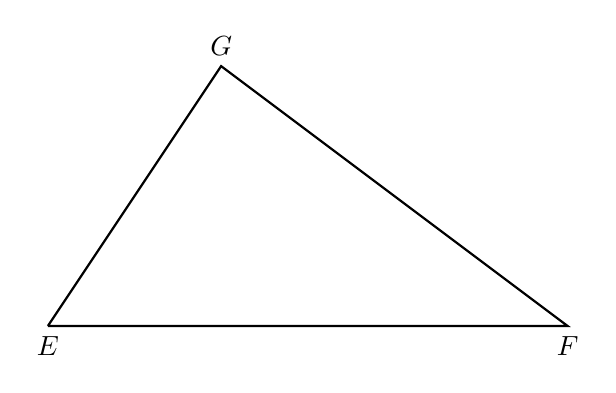
\begin{tikzpicture}[scale=1.1]
        \draw [thick]%(0,0)node[below]{$A$}--
          (2,0)node[below]{$E$}--
          (8,0)node[below]{$F$}--
          (4,3)node[above]{$G$} --(2,0);
      \end{tikzpicture}
        \vspace{2cm}
    \end{center}

  \end{multicols}
\vspace{2cm}

  \item Construct a triangle congruent to $\triangle ABC$ using the $SAS$ theorem.\\[2cm]
  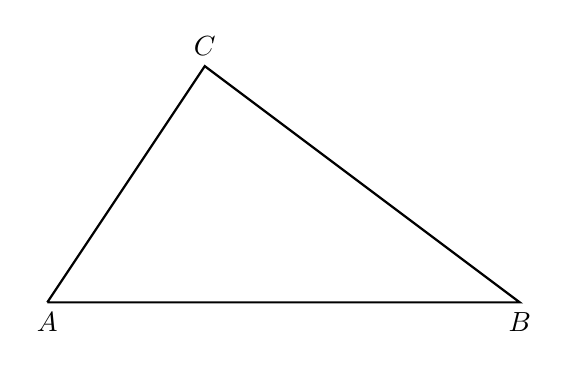
\begin{tikzpicture}%[scale=0.7]
    \draw [thick]
      (2,0)node[below]{$A$}--
      (8,0)node[below]{$B$}--
      (4,3)node[above]{$C$} --(2,0);
  \end{tikzpicture}


\end{enumerate}
\end{document}
